\label{sec:empirical}
% Empirical	Approach
% Description of the empirical model: specification and variables involved
% Strategy for the estimation of the parameters of interest and test of the hypothesis
\subsection{Baseline model}
\label{subsec:e_model}
Our baseline model is a Random Effects (RE) model to be estimated using feasible Generalized Least Squares (fGLS) where electricity consumption $e$ for grid company $i$ at time $t$ (date by hour) is given by:
\begin{equation}
  \label{eq:baseline}
  \begin{split}
  \ln e_{it}=&\ \varepsilon \widehat{\ln p_{rt}}+\delta\ln n_{im}+\bm{w}^{'}_{rt}\lambda\\
  &+\gamma\ days+\eta_{year}+\eta_{week}+\eta_{hour}\cdot\eta_{month}+\eta_{hour}\cdot\eta_{day}+c_i+u_{it}
  \end{split}
\end{equation}
where $p$ is the electricity spot price in price region $r$ at time $t$, $n$ is the number of meters at the beginning of the month $m$, $\bm{w}$ is a vector of weather variables for the given price region $r$ at time $t$ (see section \ref{subsec:d_weather}). The time variables in the second line include the time trend $days$ and the $\eta$'s representing dummies for each year and each ISO week number, as well as dummies for hour of the day interacted with month and day of the week respectively. The composite error term consists of the grid-specific time-constant unobserved effect $c_i$ that is treated as random and the idiosyncratic error $u_{it}$.
\medskip\\
We use a log-log specification for electricity consumption, the spot price, and the number of meters as it allows us to model demand responses across grid areas of different size. Furthermore, log-log is the more standard specification which allows for a more direct comparison to the results in other studies \citep{burke2017price}. Other attractive properties include that the estimation provides the elasticity directly and prevents predicting non-positive electricity consumption. Furthermore, the specification reduces the impact of outliers and is found to reduce systematic patterns in the estimated residuals \citep{burke2017price}.


\subsection{Instrumenting for prices}
\label{subsec:e_instrumenting}
To circumvent the simultaneity problem that higher expected consumption reflects in higher demand in the day-ahead-market which drives the spot price up, we instrument for the price using the wind-power production. This makes sense as the marginal cost of wind-power production is close to zero, such that a higher expected wind-power production will drive down the price due to the merit order effect as illustrated in figure \ref{fig:merit}. This inverse relationship is consistent with what we observe in our data as seen in figure \ref{fig:wp_price_dk1_week} for DK1 and in figure \ref{fig:wp_price_dk2_week} for DK2 (appendix \ref{app:data}). This insinuates that it is a relevant instrument. The instrument is also likely to be a valid one; weather is exogenous and it seems unlikely that consumption of electricity responds to wind weather through other channels than through the price of electricity conditional on temperatures and daytimes. These assumptions are tested formally in section \ref{subsec:r_validity}.
\medskip\\
As the general level of wind power production is very different between the two price regions, we expect different slopes as well which we get by interacting it with dummies for each price region, thus, we estimate the reduced form for log price $\widehat{\ln p}$ in region $r$ at time $t$ by wind power prognosis $wind$ for the same price region and time as well as using the same controls as in equation (\ref{eq:baseline}) though we expect $\underline{\delta}$ to be insignificant.
\par
Thus, estimating electricity consumption by a Random Effects Instrumental Variables (REIV) estimation is a three-stage approach starting by estimating the reduced form for log price using a Generalized IV (GIV) estimator for the pooled sample (see subsection \ref{subsec:e_re} below):
\begin{equation}
  \label{eq:reduced}
  \begin{split}
    \ln p_{r} &= (\pi_1 DK1+\pi_2 DK2)\cdot wind_{rt} +\underline{\delta}\ln n_{im}+\bm{w}^{'}_{r}\underline{\lambda}\\
  &+\underline{\gamma}\ days+\underline{\eta_{year}}+\underline{\eta_{week}}+\underline{\eta_{hour}\cdot\eta_{month}}+\underline{\eta_{hour}\cdot\eta_{day}}+v_{i}
  \end{split}
\end{equation}
\vspace{-1em}
\begin{figure}[H]
  \centering
  \caption{Wind power prognosis and spot price by week (DK1)}
  \label{fig:wp_price_dk1_week}
    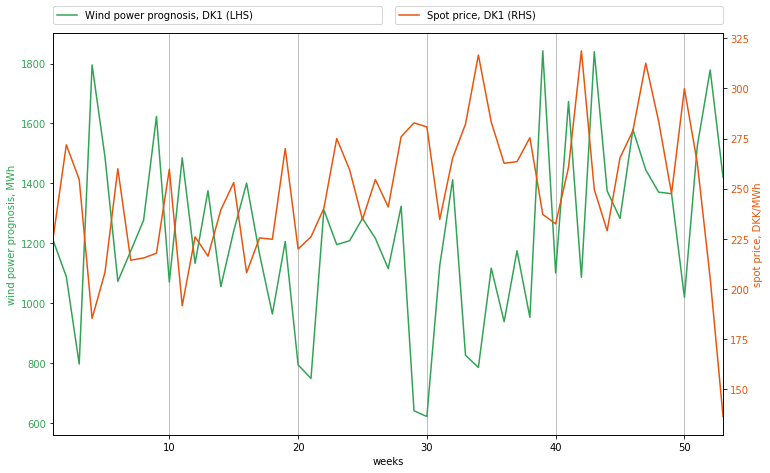
\includegraphics[width=1 \textwidth]{03_figures/wp_DK1_weeks}
\end{figure}
\noindent
An overproduction of wind power in one price region leads to transmission of cheap electricity to connected price regions, thus, as additional instruments we also consider the wind power prognosis for the other price region as well as for all of Sweden.

\subsection{Effect of Time-of-use tariff}
\label{subsec:e_tout}
To estimate the effect of the time-of-use (TOU) tariff (see subsection \ref{subsec:d_tout}) the baseline specification (\ref{eq:baseline}) is estimated for the hours 17-19 solely for the grid company Radius using pooled 2SLS (P2SLS), thus, without the grid-area unobserved effect $c_i$ but including a term for the effect of the TOU tariff:
\begin{align}
  \alpha\frac{nf_{month}}{nr_{month}}\tau_{year,month}
  \label{eq:tout}
\end{align}
Where $nf$ is the number of flex-settled meters by month, $nr$ is the total number of meters for retail customers, and $\tau$ is a dummy for being in October-March in 2018.
\medskip\\
To isolate the effect of the TOU tariff we need to assume that residual consumers do not react to the tariff so their consumption, on the contrary, is assumed to follow the same hour-by-day, hour-by-month, and week patterns as in previous years and that the effects of year dummies and the time trend are evenly distributed across the year.
\par
One weakness is that the monthly records for the number of flex-settled meters provides a lag which can result in an downward bias of $\widehat{\alpha}$ (if there is a negative effect of the tariff). This could possibly be improved by assuming a linear daily growth between $nf_{month}$ and $nf_{month+1}$.


\subsection{Random Effects estimation}
\label{subsec:e_re}
Different candidates exists for panel data estimation with unobserved effects \citep{wooldridge2010econometric}. The simplest method is \textbf{pooled ordinary least squares (POLS)} and the corresponding \textbf{pooled two stage least squares} for instrumental variables (IV) estimation in he case of endogeneity issues, which we will use for one-grid estimations of our model (\ref{eq:baseline}). The number of meters is , however, the only grid-specific background variable we have available. Thus, for full-sample estimation it is likely that the presence of unobserved heterogeneity is not controlled for and therefore correlates with the set of controls such as having different industries or firm sizes regarding wholesale or different daily patterns for retail consumers. Even if the strict exogeneity condition holds:
\begin{equation}
  cov(c_i, x_{it})=0
  \label{eq:exogeneity}
\end{equation}
then POLS would still result in serial correlation given that $c_i\neq0$, which is present in the composite error for each time period i.e. $cov(c_i+u_{it},c_i+u_{is})=\sigma_c^2>0$. Though we would still need to handle the serial correlation, a first step is to note that we regardless of estimation technique would need to use cluster robust standard errors for the full-sample estimation.
\medskip\\
Though it is a common way to handle serial correlation, we hardly consider the \textbf{first-difference (FD)} estimation as the great presence of heteroscedasticity in terms of seasonality and daily and weekly patterns with occasional holidays underlines that there is no obvious suggestion for the length of $t-s$ that would not violate the critical assumption of \eqref{eq:exogeneity}. Furthermore, we see no signs of electricity consumption acting as a unit root process in figure \ref{fig:cons_hours}.
\medskip\\
The consistent but somewhat inefficient approach is the \textbf{fixed effects (FE)} estimation as it does not assume strict exogeneity (\ref{eq:exogeneity}) due to performing a within transformation of all variables before estimating by POLS. Equivalently, \textbf{fixed effects instrumental variables (FEIV)} estimation is simply performed by within transforming both equation (\ref{eq:baseline}) and (\ref{eq:reduced}) and estimating this time-demeaned system by P2SLS. While the loss of time constant variables is a common flaw, we do not have any in our specification (\ref{eq:baseline}) except for $c_i$ that causes the serial correlation.
\medskip\\
A less extreme approach is the \textbf{random effects (RE)} estimator that first within-transform our model (\ref{eq:baseline}) to run a FE estimation in order to compute:
\begin{equation}
  \widehat{\lambda}=1-\left(\frac{\sigma^2_u}{\sigma^2_u+T\sigma^2_c}\right)^\frac{1}{2}
\end{equation}
Next we use the stored $\widehat{\lambda}$ to estimate the quasi-time demeaned system of the form:


Using the

quasi-time-demeaned system

The strict exogeneity assumption (\ref{eq:eq:exogeneity}) can be tested by the Hausman test:
\begin{equation}
  \widehat{\beta_{RE}}=\widehat{\beta_{FE}}
  \label{eq:hausman}
\end{equation}
If it holds RE is indeed more efficient than FE estimation.

26,300

\begin{itemize}
    \item Least Squares Dummy Variables estimation (LSDV)
    \begin{itemize}
        \item Unobserved heterogeneity, $\psi_i>0$, leads to serial correlation
    \end{itemize}
    \item Fixed Difference estimation (FD)
    \begin{itemize}
        \item Strict exogeneity assumption, $cov(u_{it},\bm{x}_{it})=0$, is violated by hourly-patterns
    \end{itemize}
    \item Fixed Effects estimation (FE)
    \begin{itemize}
        \item Time-demeaned, too extreme
    \end{itemize}
    \item Dynamic Panel Estimation using Generalized Methods of Moments (GMM)
    \begin{itemize}
        \item Only necessary if including lagged prices as instruments
    \end{itemize}
\end{itemize}
We choose the \textbf{Random Effects estimator (RE)} for wholesale consumption
\begin{itemize}
    \item Critical assumption for RE: No endogeneity, i.e. $cov(\psi_i,\bm{x}_{it})=0$.
    \item Hausman test: $\widehat{\beta_{RE}{*}}=\widehat{\beta_{FE}^{*}}$ no endogeneity, thus both RE and FE are consistent, but RE is more efficient.
\end{itemize}
Estimate RE estimation using \textbf{feasible Generalized Least Squares (fGLS)}
\begin{itemize}
    \item[\nth{1} stage:] Estimate eq. (\ref{eq:baseline}) using LSDV estimation $\rightarrow$ store $\widehat{\lambda}=1-\left(\frac{\sigma^2_u}{\sigma^2_u+T\sigma^2_\alpha}\right)^\frac{1}{2}$
    \item[\nth{2} stage:] LSDV using $\widehat{\lambda}$ to estimate the quasi-time demeaned system of the form: $y_{it}-\widehat{\lambda}\underline{y_i}=\beta_0(1-\widehat{\lambda})+\beta_1(\bm{x}_{it}-\widehat{\lambda}\underline{\bm{x}_i})+\psi_i(1-\widehat{\lambda})+u_{it}-\widehat{\lambda}u_{it}$.
\end{itemize}

\subsection{Robustness checks}
\label{subsec:e_robustness}
Robustness of the elasticity for wholesale electricity demand in the peak-hours 11-15 is tested by splitting the sample by price region, year, and month to look for heterogeneous effects. Furthermore, we estimate the equation (\ref{eq:baseline}) for each grid area \todo{and for the mean of each price region. As the FE estimates are identical, however less efficient, we also try to weight the estimates by the number of wholesale meters in each grid.} using P2SLS.
\par
Likewise, we estimate the elasticity for retail electricity demand in the peak-hours 17-19 by price region and year, though consumers have no price incentive to react to hourly prices except for those that become flex-settled by 2018.
\medskip\\
Tests of the robustness of the effect of the TOU tariff is less straight forward. We try including the dummy constructed for Radius in estimation of retail electricity demand in different grids.
